\documentclass[hyperref={unicode}]{beamer}
\usepackage[czech]{babel}
\usepackage{times}
\usepackage[utf8]{inputenc}
\usepackage[T1]{fontenc}
\usepackage{amsmath}
\usepackage{color}
\usetheme{Madrid}
\usecolortheme{whale}

\title{Konečné automaty}
\author[Adrián Boros]{Adrián Boros\texorpdfstring{\\ \texttt{xboros03@stud.fit.vutbr.cz}}{}}
\institute[VUT FIT]
{
	Vysoké učení technické v~Brne \\
	Fakulta informačních technológií
}
\date{\today}

\begin{document}
\begin{frame}
  \titlepage
\end{frame}

\begin{frame}
\transwipe
  \frametitle{Obsah}
  \tableofcontents
\end{frame}

\section{Konečný automat}
\begin{frame}{Konečný automat}
\transwipe
\begin{itemize}
\item {\textbf {\color{red} automaton, finit state machine}}
\item abstraktný model výpočetného stroja (počítača/programu), který číta vstupní data a~na základe prečítaných symbolov prechádza z~jedného stavu do druhého
\pause
\item najčastejšie použitie:
\begin{itemize}
\item [\textendash] konštrukcia (sekvenčných) digitálnych obvodov
\begin{itemize}
\item prvý krok návrhu je zostavenie automatového modelu funkcie obvodu
\end{itemize}
\item [\textendash] programovanie
\begin{itemize}
\item konečný automat je modelom niektorých softwareových častí, je možné pomocou neho popísať chovanie ľubovoľnej SW časti
\end{itemize}
\end{itemize}
\end{itemize}
\end{frame}

\section{Formálna definícia}
\begin{frame}{Formálna definícia}
\transwipe
\begin{itemize}
\item \textbf{Konečný automat KA} je šestica $KA = \langle X, Y, Q, \delta, \lambda, Q_0\rangle$, kde:
\begin{itemize}
\pause
\item ${X}$ je vstupná abeceda (konečná množina vstupných písmen),
\item ${Y}$ je výstupná abeceda (konečná množina výstupných písmen),
\item $Q$ je konečná množina vnútorných stavov
\item $\delta$ je stavovo prechodová funkcia, $X \times Q\longrightarrow Q$
\item $\lambda$ je výstupná funkcia, $X \times Q \longrightarrow Y$
\item $Q_0 \in Q$ je počiatočný vnútorný stav
\end{itemize}
\end{itemize}
\end{frame}

\section{Varianty automatov}
\begin{frame}{Varianty automatov}
\transwipe
\begin{itemize}
\pause
\item \textbf{Medvedeov automat}
\begin{itemize}
\pause
\item [\textendash] nemá množinu výstupných písmen ani definovanú výstupnú funkciu
zpracovaní vstupnej postupnosti nás zaujíma, v~akom vnútornom stave sa automat nachádza (tzv. transducer)
\item [\textendash] tento model sa využíva ako napr. lexikálny analyzátor v~prekladačoch programovacích jazykov
\end{itemize}
\pause
\item \textbf {Autonómny automat}
\begin{itemize}
\pause
\item [\textendash] nemá množinu vstupných písmen a~prechody sú definované len \uv{zo stavu do stavu}: $Q_{t+1}=\delta(Q_t)$
\item [\textendash] takýto automat môže byť modelom pri návrhu autonómnych čítačov
\end{itemize}
\end{itemize}
\end{frame}

\begin{frame}
\transwipe
\begin{itemize}
\item \textbf{Stochastický automat}
\begin{itemize}
\item [\textendash] má definované jednotlivé prechody pomocou pravdepodobnosti
\end{itemize}
\item \textbf{Fuzzy automat}
\begin{itemize}
\item [\textendash] stavovo prechodová a~výstupná funkcia sú definované pomocou operácií fuzzy logiky 
\item [\textendash] stavy, vstupy a~výstupy sú definované ako fuzzy množiny 
\end{itemize}
\end{itemize}
\end{frame}

\section{Zobrazovanie automatov}
\begin{frame}{Zobrazovanie automatov}
\transwipe
\begin{itemize}
\pause
\item \textbf{grafom prechodov a výstupov}
\begin{itemize}
\pause
\item [\textendash] orientovaný graf
\item [\textendash] uzly = stavy, hrany = prechody medzi stavmi
\item [\textendash] Mooreov automat
\begin{itemize}
\item ohodnotenie hrán: vstupy: podmienky prechodu
\item ohodnotenie uzlov: výstupy odpovedajúce stavom
\end{itemize}
\item [\textendash] Mealyho automat
\begin{itemize}
\item ohodnotenie hrán: vstupy\,--\,podmienky prechodu a~výstupy
\end{itemize}
\end{itemize}
\pause
\item \textbf{tabuľkou prechodov a~výstupov}
\end{itemize}
\end{frame}

\begin{frame}
\transwipe
\begin{itemize}
\item Automat vyjadrený vo forme tabuľky prechodov a~výstupov
\end{itemize}
\begin{table}[h]
\centering
\begin{tabular}{|c|c|c|c|}
\hline
   & 0  & 1  & Y \\ \hline
$Q_0$ & $Q_0$ & $Q_1$ & 0 \\ \hline
$Q_1$ & $Q_0$ & $Q_2$ & 1 \\ \hline
$Q_2$ & $Q_0$ & $Q_2$ & 0 \\ \hline
\end{tabular}
\end{table}
\begin{itemize}
\item Automat vyjadrený pomocou grafu
\begin{figure}[h]
\centering
\scalebox{0.7}{
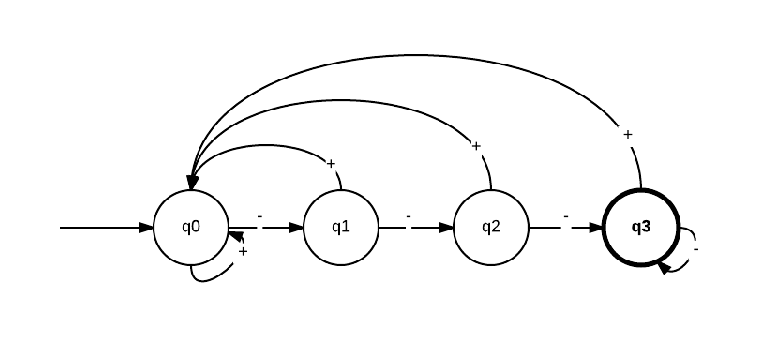
\includegraphics{automat.eps}}
\end{figure}
\end{itemize}
\end{frame}

\section{Mooreov konečný automat}
\begin{block}{Mooreov konečný automat}
\transwipe
\begin{itemize}
\item jednoduché zariadenie s~konečným počtom vnútorných stavov, medzi ktorými se prechádza na základe vstupných symbolov
\item každý vnútorný stav má definovanú práve jednu hodnotu na výstupu
\item automat musí mať definovaný východzí stav, v~ktorom sa nachádza pred zadáním prvého vstupného symbolu
\end{itemize}
\end{block}
\begin{figure}[h]
\centering
\scalebox{0.65}{
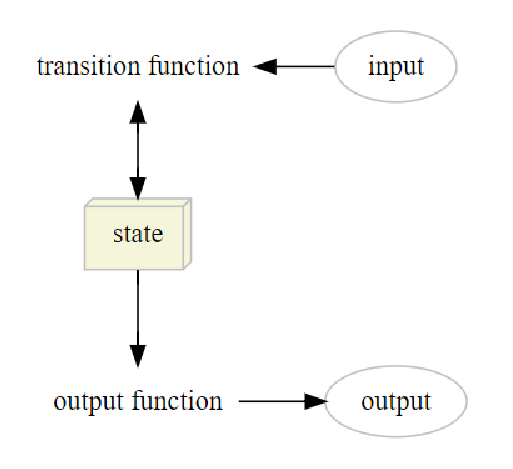
\includegraphics{moore.eps}}
\end{figure}

\section{Mealyho konečný automat}
\begin{block}{Mealyho konečný automat}
\transwipe
\begin{itemize}
\item zobecnenie Moorovho konečného automatu
\item líši se len tým, že výstup nezávisí len na vnútornom stave, ale i~na vstupe
\item vo formálnej definícii se táto odlišnosť prejavuje iným definičným oborom výstupnej funkcie
\end{itemize}
\end{block}
\begin{figure}[h]
\centering
\scalebox{0.75}{
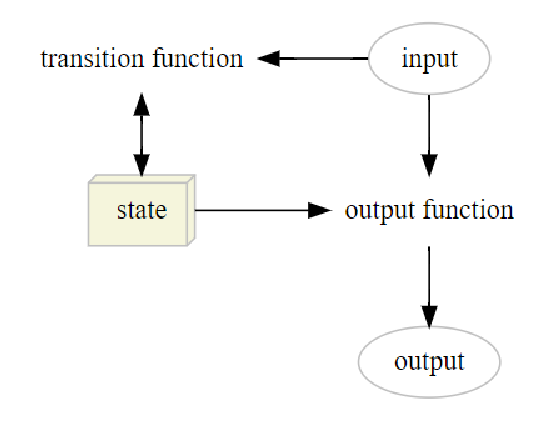
\includegraphics{mealy.eps}}
\end{figure}


\section{Implementácia}
\begin{frame}{Implementácia}
\transwipe
\begin{itemize}
\item softwarovo sa konečný automat implementuje takto:
\begin{itemize}
\item vnútorný stav ukladáme do premennej, spravidla výčtového dátového typu
\item činnosť automatu predstavuje cyklus s~príkazom vetvenia v~jeho tele
\begin{itemize}
\item najprv sa prepíname podľa stavov a~potom podľa vnútorných premenných
\end{itemize}
\end{itemize}
\end{itemize}
\end{frame}

\begin{frame}{Použitá literatúra}
\transwipe
\begin{thebibliography}{10}
\bibitem[Konečný automat]{automat} Konečný automat
\newblock {\texttt{https://matematika.cz/konecny-automat}
\texttt{http://slideplayer.cz/slide/3442954/}
\texttt{http://voho.eu/wiki/konecny-automat/}}
\bibitem[Mealyho automat]{Mealy} Mealyho automat
\newblock \texttt{http://voho.eu/wiki/mealy/}
\bibitem[Mooreov automat]{Moore} Mooreov automat
\newblock \texttt{http://voho.eu/wiki/moore/}
\end{thebibliography}
\end{frame}
\end{document}